\documentclass[20pt,margin=0.9in,innermargin=-4.5in,blockverticalspace=-0.25in]{tikzposter}
\geometry{paperwidth=43in,paperheight=32.5in}
\usepackage[utf8]{inputenc}
\usepackage{amsmath}
\usepackage{amsfonts}
\usepackage{amsthm}
\usepackage{amssymb}
\usepackage{mathrsfs}
\usepackage{graphicx}
\usepackage{adjustbox}
\usepackage{enumitem}
\usepackage{wrapfig}
\usepackage[backend=biber,style=numeric]{biblatex}
\usepackage{SUtheme}

\usepackage{mwe} % for placeholder images

\usepackage{comment}

\addbibresource{refs.bib}

% set colored boxes
\usepackage[most]{tcolorbox}
\newtcolorbox{definitionBox}{
  colback=blue!10,
  colframe=blue!50!black,
  fonttitle=\bfseries,
  title=Definition,
  arc=3mm,
  boxrule=0.8pt
}

\newtcolorbox{theoremBox}{
  colback=teal!10,
  colframe=teal!50!black,
  fonttitle=\bfseries,
  title=Theorem,
  arc=3mm,
  boxrule=0.8pt
}

\newtcolorbox{exampleBox}{
  colback=cyan!10,
  colframe=cyan!50!black,
  fonttitle=\bfseries,
  title=Example,
  arc=3mm,
  boxrule=0.8pt
}

% set theme parameters
\tikzposterlatexaffectionproofoff
\usetheme{SUTheme}
\usecolorstyle{SUStyle}
\usetitlestyle{Filled}

\usepackage[scaled]{helvet}
\renewcommand\familydefault{\sfdefault} 
\usepackage[T1]{fontenc}

\linespread{0.8}

\title{Lie Algebra of a Lie Group}
\author{Zih-Yu Hsieh \quad\quad Mentor: Arthur Jiang}
\institute{University of California Santa Barbara}
\titlegraphic{
\includegraphics[width=0.06\textwidth]{logo.png}}

% begin document
\begin{document}
\maketitle
\centering
\begin{columns}
    \column{0.32}
    \block{Tangent Vectors as Derivations}{
        \vspace*{-1em}
        When embedding smooth manifolds into $\mathbb{R}^n$, tangent vectors are associated with directional derivatives. To generalize tangent vectors into abstract smooth manifold, we need an analogy:
        
        \begin{definitionBox}
            Any point $u\in M$, a \textbf{Derivation at $u$}, is a linear map $v_u:C^\infty(M)\rightarrow\mathbb{R}$, that satisfies the product rule:
            $$\forall f,g\in C^\infty(M),\quad v_u(fg) = f(u)(v_u g)+g(u)(v_u f)$$ 
            The vector space of all derivations at $u$, or $T_u(M)$, is the \textbf{Tangent Space} of $M$ at $u$, and each derivation $v_u\in T_u(M)$ is a \textbf{Tangent Vector} of $u$.
        \end{definitionBox}
    }
    \block{Vector Fields \& Smooth Condition}{
        \vspace*{-1em}
        \begin{definitionBox}
            a vector field is a map $X:M\rightarrow TM$ ($TM$ denotes the \textbf{Tangent Bundle}), with $X(u) = X_u\in T_u(M)$.

            Which, $X$ is a \textbf{Smooth Vector Field}, if $X:M\rightarrow TM$ is a smooth map. 
            
            A collection of smooth vector fields on $M$ is denoted as $\mathfrak{X}(M)$, which is an $\mathbb{R}$-vector space.
        \end{definitionBox}

        An equivalent condition of saying a vector field $X$ is smooth, is through smooth functions $f\in C^\infty(M)$: For all $u\in M$, $X(u)= X_u\in T_u(M)$ is a derivation at $u$, define $Xf:M\rightarrow\mathbb{R}$ by $Xf(u) = X_u(f)$, then $X$ is a smooth vector field iff $Xf\in C^\infty(M)$. Which, a smooth vector field can be viewed as a \textbf{Derivation:}
        \begin{theoremBox}
            For all $f,g\in C^\infty(M)$, given $X\in\mathfrak{X}(M)$, any $u\in M$ satisfies product rule:
            $$X(fg)(u) = X_u(fg) = f(u)(X_ug) + g(u)(X_uf) = f(u)Xg(u)+g(u)Xf(u)$$
            $$\implies X(fg) = f(Xg) + g(Xf)$$
        \end{theoremBox}
    }
    \block{Vector Fields of Different Manifolds}{
        \vspace*{-1em}
        Given $M,N$ two smooth manifolds, and smooth map $F:M\rightarrow N$. Let $X\in\mathfrak{X}(M)$, an ideal situation is mapping $X$ to a smooth vector field of $N$ through $F$. Yet, this requires $F$ to be bijective:
        
        \begin{center}
            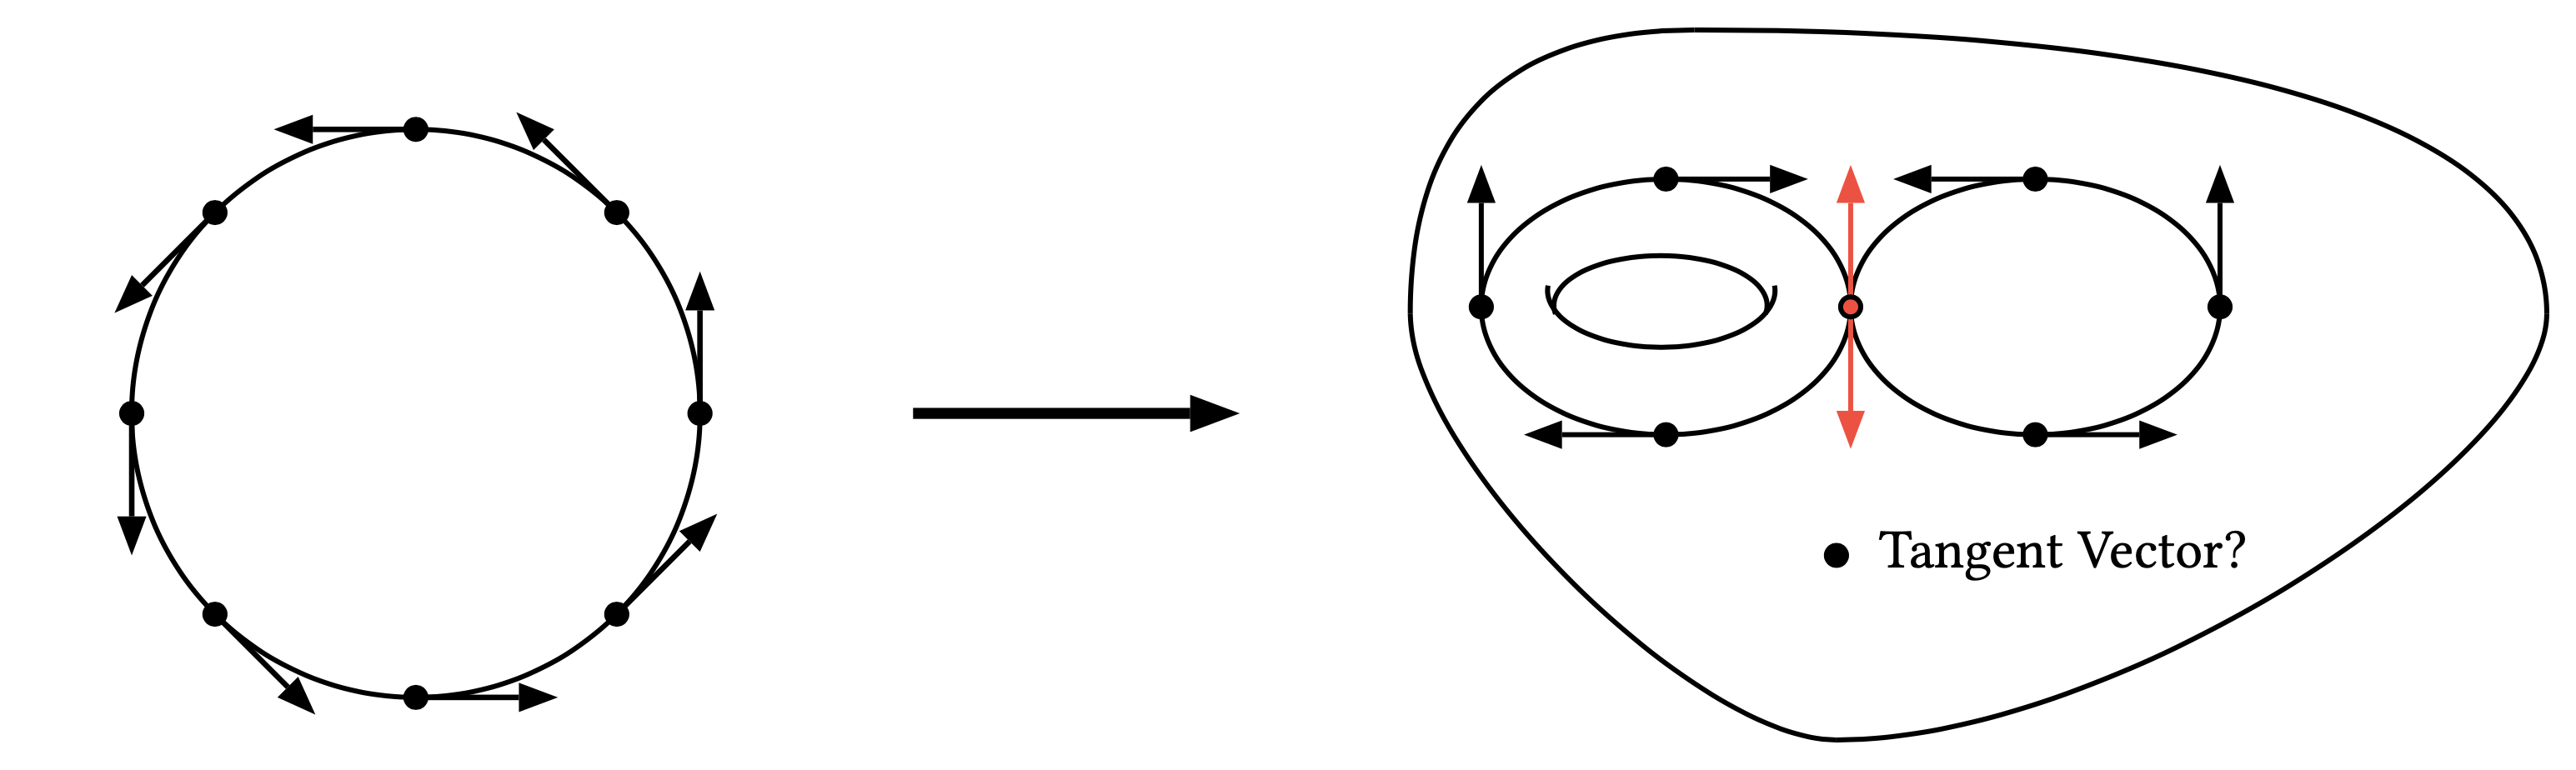
\includegraphics[width=0.24\textwidth]{example 1.png} 

            \textbf{Figure 1:} Example of Conflicting Tangent Vectors
        \end{center}

        \hfil

        So, we'll consider a weaker notion: 
        \begin{definitionBox}
            Given $X\in\mathfrak{X}(M)$ and $Y\in\mathfrak{X}(N)$, the two are $\boldsymbol{F}$\textbf{-related}, if for all $u\in M$, the following is true:
            $$dF_u(X_u) = Y_{F(u)}$$
            Simply speaking, $F$ maps the tangent vectors collected by $X$, to be compatible with tangent vectors collected by $Y$.
        \end{definitionBox}

        \begin{center}
            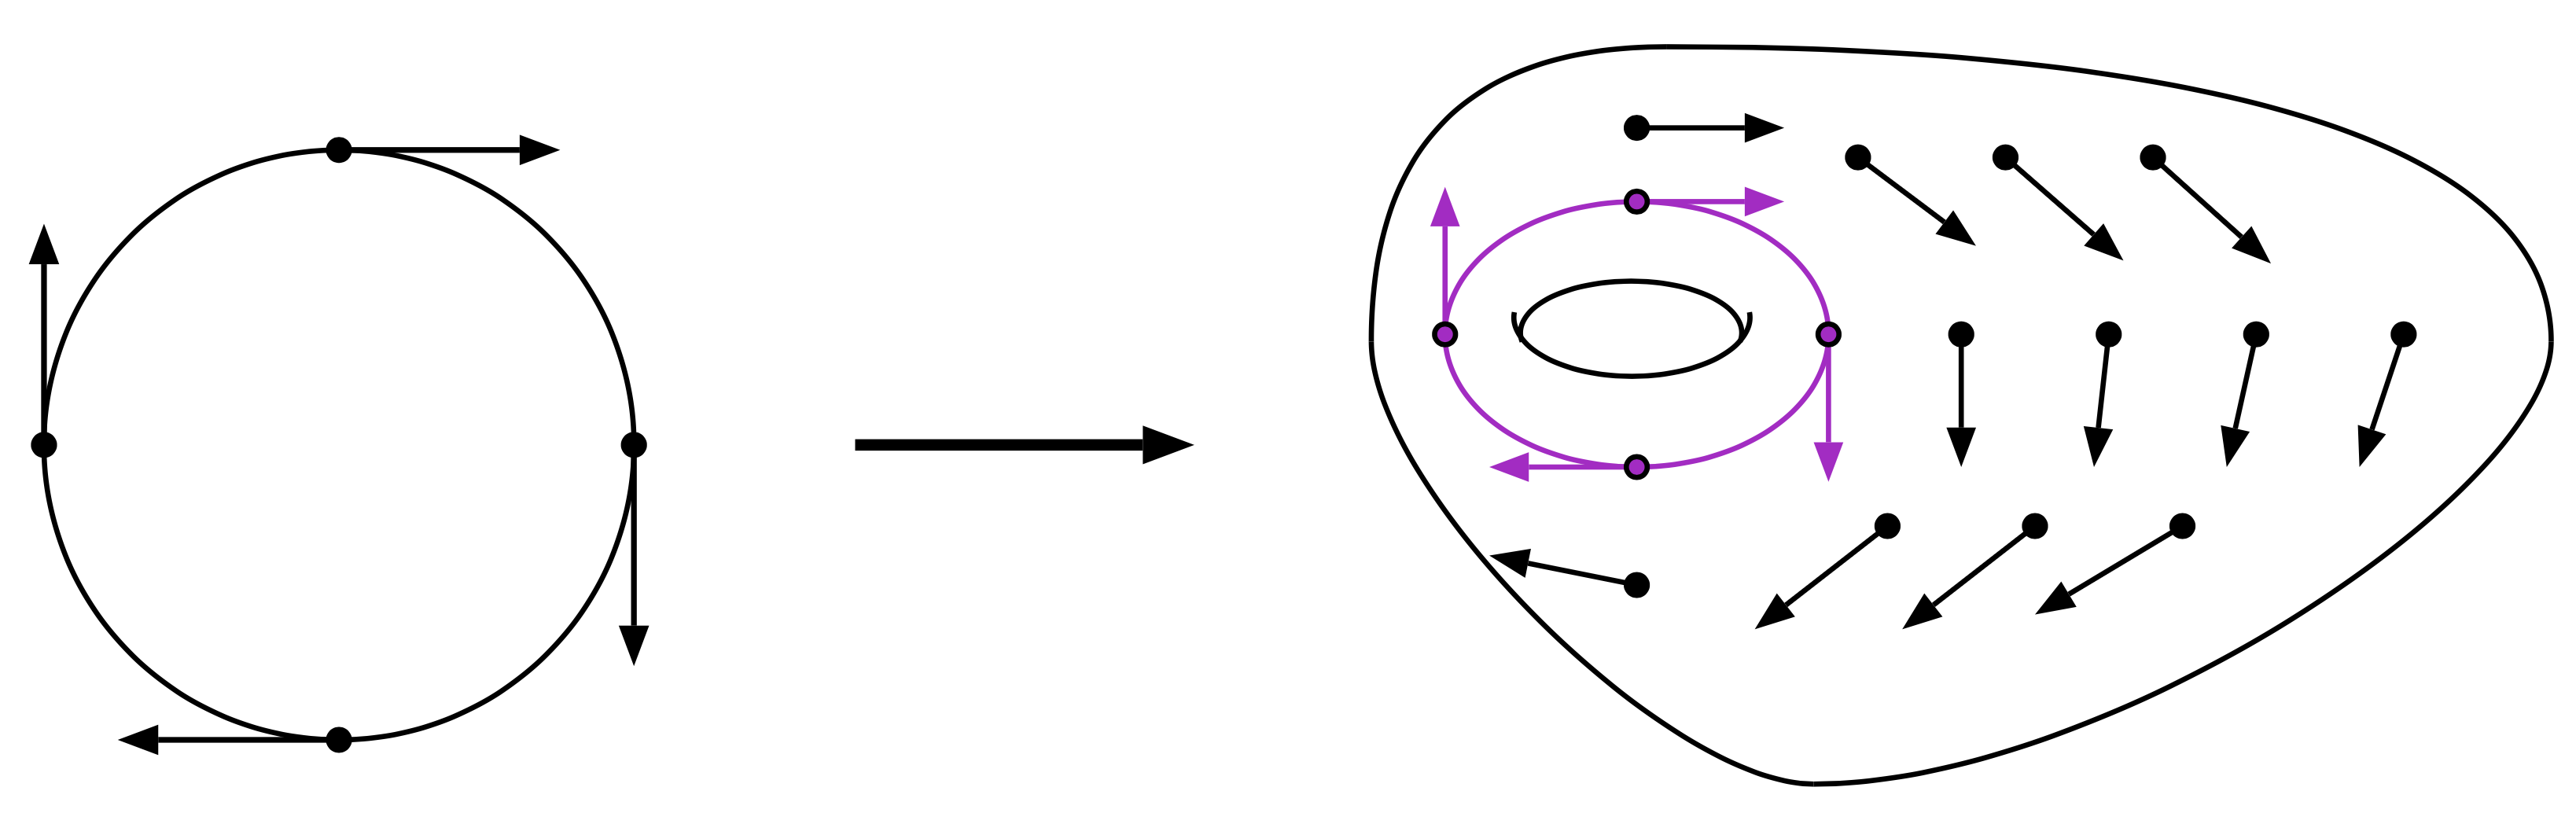
\includegraphics[width=0.24\textwidth]{example 2.png} 

            \textbf{Figure 2:} A demonstration of $F$-Relation
        \end{center}
    }

    \column{0.36}

    \block{Lie Bracket of Vector Fields}{
        \vspace*{-1em}
        The initial motivation is to combine two vector fields $X,Y\in \mathfrak{X}(M)$ to be another vector field. For all $f\in C^\infty(M)$, since $Yf\in C^\infty(M)$, then $XYf := X(Yf)\in C^\infty(M)$. But, in general $XY$ is not a derivation, hence not a vector field:
        \begin{exampleBox}
            Define vector fields $X=\frac{\partial}{\partial x}$, $Y=x\frac{\partial}{\partial y}$ on $\mathbb{R}^2$. Take smooth functions $f(x,y)=x$ and $g(x,y)=y$, then we get the following:
            $$XY(fg) = X\left(x\frac{\partial}{\partial y}(xy)\right) = \frac{\partial}{\partial x}(x^2) = 2x$$
            But, product rule doesn't hold for this example:
            $$f(XY g)+g(XY f)=x\left(X\left(x\frac{\partial}{\partial y}(y)\right)\right) + y\left(X\left(x\frac{\partial}{\partial y}(x)\right)\right) = x$$
        \end{exampleBox}
        So, we need to define a new operation on vector fields: 
        \begin{definitionBox}
            The \textbf{Lie Bracket} $[\cdot,\cdot]:\mathfrak{X}(M)\times \mathfrak{X}(M)\rightarrow \mathfrak{X}(M)$, is defined as:
        $$\forall X,Y\in\mathfrak{X}(M),\quad [X,Y]=XY-YX$$
        Which, the output $[X,Y]\in\mathfrak{X}(M)$, since it satisfies product rule:
        $$[X,Y](fg) = X(Y(fg))-Y(X(fg))= X(f(Yg)+g(Yf))-Y(f(Xg)+g(Xf))$$
        $$ = f(XYg)+(Yg)(Xf)+g(XYf)+(Yf)(Xg)-f(YXg)-(Xg)(Yf)-g(YXf)-(Xf)(Yg)$$
        $$ = f(XYg-YXg)+g(XYf-YXf) = f[X,Y](g)+g[X,Y](f)$$
        Lie Bracket also satisfies these properties:
        \begin{itemize}
            \item \textbf{Bilinearity:} $[aX+bY,Z]=a[X,Z]+b[Y,Z]$
            \item \textbf{Antisymmetry:} $[X,Y]=-[Y,X]$
            \item \textbf{Jacobi's Identity:} $\left[X,[Y,Z]\right]+ \left[Y,[Z,X]\right]+ \left[Z,[X,Y]\right]=0$
        \end{itemize}
        \end{definitionBox}
        Moreover, Lie Bracket inherits relation of smooth maps:
        \begin{theoremBox}
            Given smooth map $F:M\rightarrow N$, if $X_1,X_2\in\mathfrak{X}(M)$ and $Y_1,Y_2\in\mathfrak{X}(N)$ are $F$-related respectively, then $[X_1,X_2]\in \mathfrak{X}(M)$ and $[Y_1,Y_2]\in\mathfrak{X}(N)$ are also $F$-related. 
        \end{theoremBox}
    }
    \block{Lie Groups \& Left-Invariant Vector Fields}{
        \vspace*{-1em}
        The initial motivation is to study group structures in some smooth manifolds.
        
        \begin{definitionBox}
            A \textbf{Lie Group} $G$, is a smooth manifold along with group structure, such that the group operation $P:G\times G\rightarrow G$ by $P(g,h) = gh$, and the inversion map $i:G\rightarrow G$ by $i(g)=g^{-1}$ are both smooth maps between manifolds.
        \end{definitionBox}

        For all $g\in G$, denote the left multiplication $L_g:G\rightarrow G$ by $L_g(h)=gh$,
        since $L_g = P\bigm|_{\{g\}\times G}$, it is a smooth map. Hence, there's a notion of $X$ being $L_g$-related to itself:

        \begin{definitionBox}
            Given any $X\in\mathfrak{X}(G)$ and all $g\in G$, $X$ is a \textbf{Left-Invariant Vector Field}, if for all $g\in G$, $X$ is $L_g$-related to itself. Which, for all $g\in G$: 
            $$d(L_g)_e(X_e) = X_{L_g(e)} = X_g$$ 
            So, $X$ is uniquely determined by its tangent vector at identity, $X_e\in T_e(G)$.

            The collection of Left-Invariant vector fields $\mathfrak{g}\subseteq \mathfrak{X}(G)$, is a linear subspace. 
            
            %Also, as vector spaces, $\mathfrak{g}\cong T_e(G)$.
        \end{definitionBox}

        Recall that Lie Bracket of vector field preserves $F$-relation between manifolds, so:
        \begin{theoremBox}
            For all $X,Y\in\mathfrak{X}(G)$ that are left-invariant, since for all $g\in G$, $X$ and $Y$ are $L_g$ related to themselves, then the Lie Bracket $[X,Y]$ is also $L_g$-related to $[X,Y]$. Hence, $[X,Y]$ is also left-invariant, so $\mathfrak{g}$ is closed under Lie Bracket's operation.
        \end{theoremBox}
    }

    \column{0.32}
    \block{Lie Algebra on a Lie Group}{
        \vspace*{-1em}
        \begin{definitionBox}
            Given a vector space $\mathfrak{g}$ over $\mathbb{R}$ or $\mathbb{C}$, with a binary operation $[\cdot,\cdot]:\mathfrak{g}\times \mathfrak{g}\rightarrow \mathfrak{g}$, such that the following holds:
            \begin{itemize}
                \item \textbf{Bilinearity:} $[aX+bY,Z]=a[X,Z]+b[Y,Z]$
                \item \textbf{Antisymmetry:} $[X,Y]=-[Y,X]$
                \item \textbf{Jacobi's Identity:} $\left[X,[Y,Z]\right]+\left[Y,[Z,X]\right]+\left[Z,[X,Y]\right]=0$
            \end{itemize}
            Then, the pair $(\mathfrak{g},[\cdot,\cdot])$ is a \textbf{Lie Algebra}.
        \end{definitionBox}
        In general, Lie Algebra is non-associative, so Jacobi's Identity is an alternative condition. Finally, we can define \textbf{Lie Algebra of a Lie Group:}
        \begin{definitionBox}
            Given a lie group $G$, since the subset of left-invariant vector fields $\mathfrak{g}\subseteq \mathfrak{X}(G)$ forms a linear subspace, while closed under Lie Bracket's operation, then the pair $(\mathfrak{g},[\cdot,\cdot])$ forms a \textbf{Lie Algebra} of $G$, denoted as $Lie(G)$.
        \end{definitionBox}

        Here's an example of Lie Algebra on a Lie Group:

        \begin{exampleBox}
            \textbf{General Linear Group \& its Lie Algebra:}
            
            Given $GL_n(\mathbb{R})\subset M_n(\mathbb{R})$, since $M_n(\mathbb{R})\cong \mathbb{R}^{n^2}$ and $GL_n(\mathbb{R})$ is an open subset, it's a smooth manifold with dimension $n^2$.
            
            Which, the product of matrices and inversion are smooth functions, so $GL_n(\mathbb{R})$ is a Lie Group.

            Now, consider $\mathfrak{g}=Lie(GL_n(\mathbb{R}))$: Each Left-Invariant vector field $X\in\mathfrak{g}$ is uniquely characterized by $X_{I_n}\in T_{I_n}(GL_n(\mathbb{R}))$. In fact, such characterization is a 1-to-1 correspondance. So, as vector spaces, $\mathfrak{g}\cong T_{I_n}(GL_n(\mathbb{R}))$.

            \hfil

            \textbf{Lie Algebra on $M_n(\mathbb{R})$:}

            Given $M_n(\mathbb{R})$ as $\mathbb{R}$-vector space and the commutator $[A,B]=AB-BA$, the pair $(M_n(\mathbb{R}),[\cdot,\cdot])$ in fact forms a Lie Algebra, denoted as $\mathfrak{gl}_n(\mathbb{R})$.

            

            \hfil

            \textbf{Lie Algebra Isomorphism between $\mathfrak{g}$ and $\mathfrak{gl}_n(\mathbb{R})$:}

            $GL_n(\mathbb{R})$ has a global coordinate provided by $M_n(\mathbb{R})$, denote as $(X^i_j)_{1\leq i,j\leq n}$.
            
            For each $A\in \mathfrak{gl}_n(\mathbb{R})$, it corresponds to a tangent vector in $T_{I_n}(GL_n(\mathbb{R}))$:
            $$A = (A^i_j)\mapsto A^i_j\frac{\partial}{\partial X^i_j}\bigg|_{I_n}$$
            Which, the above tangent vector defines a Left-Invariant vector field $A^L\in \mathfrak{g}$. For all $X\in \mathfrak{g}$, the left multiplication $L_X$ provides the following relation:
            $$A^L_X=d(L_X)_{I_n}\left(A^i_j\frac{\partial}{\partial X^i_j}\bigg|_{I_n}\right) = X^i_j A^j_k\frac{\partial}{\partial X^i_k}\bigg|_{X},\quad A^L=X^i_j A^j_k\frac{\partial}{\partial X^i_k}$$
            Which, for arbitrary $A,B\in\mathfrak{gl}_n(\mathbb{R})$, Lie Bracket of $A^L,\ B^L\in\mathfrak{g}$ generates:
            $$\left[A^L,B^L\right] = X^i_jA^j_k\frac{\partial}{\partial X^i_k}(X^p_qB^q_r)\frac{\partial}{\partial X^p_r}-X^p_qB^q_r\frac{\partial}{\partial X^p_r}(X^i_jA^j_k)\frac{\partial}{\partial X^i_k}$$
            Which, each $A^j_k,\ B^q_r$ are constants, while $\frac{\partial}{\partial X^i_k}X^p_r = 1$ iff $(i,k)=(p,r)$ and is $0$ otherwise. Then, match $j=q$ for the same intermediate index, we get:
            $$\left[A^L,B^L\right] = X^i_j(A^j_kB^k_r-B^j_kA^k_r)\frac{\partial}{\partial X^i_r} = (AB-BA)^L=[A,B]^L$$
            Hence, $\mathfrak{gl}_n(\mathbb{R})$ and $\mathfrak{g}$ are isomorphic as Lie Algebra, since $A\mapsto A^L$ preserves Lie Bracket.
        \end{exampleBox}
    }

   \block{Acknowledgements \& Reference}{
        \vspace*{-1em}
        I want to thank my mentor Arthur Jiang for the effort and insights on the materials and this project, as well as UCSB Math DRP for this opportunity. 

        \hfil

        \textrm{\textbf{Reference:} Lee, J.M. \textit{Introduction to Smooth Manifolds}; 2nd ed.; Springer: New York, 2012; 9781441999825}
    }
\end{columns}
\end{document}